\documentclass[a4paper,12pt]{article}
\usepackage{a4wide}
\usepackage{tikz}
\usetikzlibrary{calc}

\begin{document}
\pagestyle{empty}
\setlength{\parindent}{0em} 
\section*{ALU}

Your task is to program the behavior of an entity called "ALU". This entity is declared in the attached file "ALU.vhdl" and has the following properties:
\begin{itemize}
\item Inputs: Clk and enable with type std\_logic; these are clock cycle and enable signals
\item Inputs: A and B with type std\_logic\_vector; these are operants
\item Inputs: slc with type std\_logic\_vector; this is a selector for choosing one of operators
\item Outputs: R with type std\_logic\_vector; this is the output of operation with the same length as inputs
\item Outputs: flag with type std\_logic; this is one-bit flag
\end{itemize}
\vspace{0.3cm}
\begin{center}
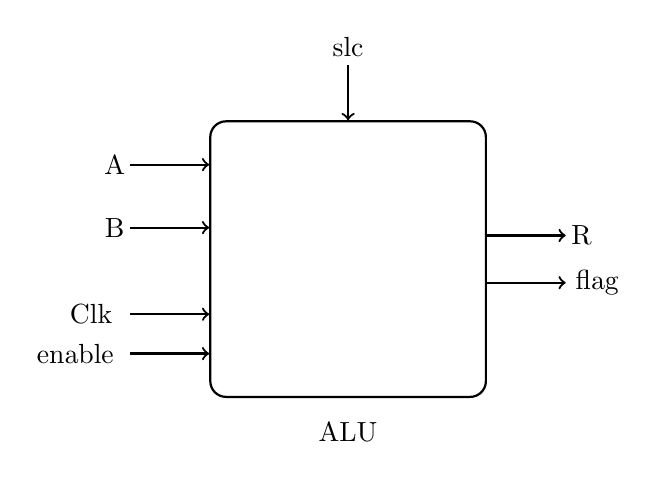
\begin{tikzpicture}
\draw node [draw,rectangle, minimum height=35mm, minimum width=35mm,rounded corners=2mm,thick](entity){};
\draw[->,thick] ($ (entity.west)-(10mm,-12mm)$) -- ($ (entity.west) - (0mm,-12mm)$);
\draw node at ($ (entity.west)-(12mm,-12mm)$){A};
\draw[->,thick] ($ (entity.west)-(10mm,-4mm)$) -- ($ (entity.west) - (0mm,-4mm)$);
\draw node at ($ (entity.west)-(12mm,-4mm)$){B};

\draw[->,thick] ($ (entity.west)-(10mm,7mm)$) -- ($ (entity.west) - (0mm,7mm)$);
\draw node at ($ (entity.west)-(15mm,7mm)$){Clk};
\draw[->,thick] ($ (entity.west)-(10mm,12mm)$) -- ($ (entity.west) - (0mm,12mm)$);
\draw node at ($ (entity.west)-(17mm,12mm)$){enable};

\draw[->,thick] ($ (entity.east) + (0mm,-3mm)$) -- ($ (entity.east) + (10mm,-3mm)$);
\draw node at ($ (entity.east) + (14mm,-3mm)$){flag};
\draw[->,thick] ($ (entity.east) + (0mm,3mm)$) -- ($ (entity.east) + (10mm,3mm)$);
\draw node at ($ (entity.east) + (12mm,3mm)$){R};

\draw[->,thick] ($ (entity.north) + (0mm,7mm)$) -- (entity.north) ;
\draw node at ($ (entity) + (0mm,27mm)$){slc};


\draw node at ($ (entity) - (0,22mm)$){ALU};

\end{tikzpicture}
\end{center}

Do not change the file "ALU.vhdl".
\\

The "ALU" entity shall behave according to the following ALU:
\\
it has two input data which we assume that they are unsigned, a clock cycle, enable signal and a selector to select which instructions has to be performed. The length of data is 4 bits. The clock cycle is active high, and instruction set includes %%INS1, %%INS2, %%INS3 and %%INS4. The value of selector for each instruction is as follow:
\\
\begin{itemize}
\item "00": %%INS1
\item "01": %%INS2
\item "10": %%INS3
\item "11": %%INS4
\end{itemize}
\vspace{0.3cm}

The instruction description is as below:
\begin{itemize}
\item %%INS1: %%DESC1 
\item %%INS2: %%DESC2
\item %%INS3: %%DESC3
\item %%INS4: %%DESC4
\end{itemize}
\vspace{0.3cm}

When the ALU is disabled, the outputs are zero and when it is enabled it performs the selected instruction on the inputs and then outputs the result. The result is as the same size as the input. There is also another output which is one-bit flag and should be calculated for each selected operation. The flag for each instruction is as follow:
\begin{itemize}
\item %%INS1: %%FLAG1 
\item %%INS2: %%FLAG2
\item %%INS3: %%FLAG3
\item %%INS4: Carry flag changes during the operation (based on the above description)
\end{itemize}
\vspace{0.3cm}

This behavior has to be programmed in the attached file "ALU\_beh.vhdl". 
\\

To turn in your solution, write an email to %%SUBMISSIONEMAIL with Subject "Result Task %%TASKNR" and attach your file "ALU\_beh.vhdl".

\vspace{0.7cm}

Good Luck and May the Force be with you.



\end{document}\grid\grid
